\section{(Integral) Affine Manifolds}

\begin{frame}[c]{Affine Manifolds}

	\begin{kulblock}{Definition}
		An \textit{affine manifold} is a differentiable manifold such that the transition maps lie in the affine group $\text{Aff}(\R^n)$
	\end{kulblock}
	\begin{remark}
		The group $\text{Aff}(\R^n) := \text{GL}(\R^n) \ltimes \R^n$. An element $g \in \text{Aff}(\R^n)$ acts on $x\in \R^n$ by $g(x) = Ax +b$ where $A \in \text{GL}(\R^n)$ and $b \in \R^n$.
	\end{remark}
\end{frame}

\begin{frame}[c]{(Integral) Affine Manifolds}

	\begin{figure}
		\includegraphics[width=0.6\textwidth]{shearGrid.png}
		\caption{Affine shear transformation}
	\end{figure}
\end{frame}

\begin{frame}[c]{The Affine Connection}

	\begin{kulblock}{Proposition}
		An affine manifold $M$ comes equipped with a flat, torsion free connection
		$\nabla$. In affine coordinates this appears as the standard Euclidean connection.
	\end{kulblock}

	\begin{remark}
		Conversely, a manifold $M$ equipped with a flat, torsion free connection can be endowed with an affine structure.
	\end{remark}
\end{frame}

\begin{frame}[c]{The Development Pair}

	\begin{kulblock}{Lemma (C. Ehresmann)}
		Let M be an affine manifold and denote by $\tilde{M}$ its universal cover. Then there exists a pair (dev, hol) called the \textit{development pair} where
		$$ \text{dev}: \tilde{M} \to \mathbb{R}^n ,$$
		$$ \text{hol}: \pi_1(M) \to \text{Aff}(\R^n)$$
		The linear part of hol is the holonomy of the affine connection $\nabla$.
	\end{kulblock}

\end{frame}

\begin{frame}[c]{Integral Affine Manifolds}

	\begin{kulblock}{Definition}
		An \textit{integral affine manifold} is an affine manifold such that the transition maps lie in the integral affine group $\text{Aff}_{\Z}(\R^n)$ - e.g. the linear part is in $\text{GL}(\Z^n)$
	\end{kulblock}
	\begin{remark}
		An integral affine structure on a manifold $M^n$ is equivalent to a rank-$n$ lattice in $T^*M$ locally spanned by closed 1-forms
	\end{remark}
\end{frame}

\section{Completeness}
\begin{frame}[c]{Complete Affine Manifolds}

	\begin{kulblock}{Definition}
		An affine manifold is said to be complete if the development map is a global diffeomorphism. This is equivalent to completeness of the connection $\nabla$.
	\end{kulblock}
	\begin{remark}
		If a discrete group $G$ acts freely and properly on $\R^n$ by affine transformations then $\R^n/G$ will inherit a complete affine structure.
	\end{remark}
\end{frame}

\section{Classifying Integral Affine Structures}
\begin{frame}[c]{Classifying Complete Integral Affine Structures}
	\begin{itemize}
		\item Completeness forces injectivity of holonomy representation
		\item Classifying complete structures $\longleftrightarrow$ classifying injective
		      holonomy representations inducing free and proper action on $\R^n$.
	\end{itemize}
\end{frame}

\begin{frame}[c]{Possible Compact Affine Surfaces}
	\begin{kulblock}{Theorem (Milnor)}
		If M is a compact, orientable surface of genus $g\geq 2$, then it does not possess a flat affine connection.
	\end{kulblock}

	\begin{corollary}
		The only possible orientable compact surfaces admitting an (integral) affine structure are sphere $S^2$ and the torus $T^2$
	\end{corollary}
\end{frame}

\begin{frame}[c]{Possible Compact Affine Surfaces}
	\begin{kulblock}{Lemma}
		$S^2$ does not admit an (integral) affine structure
	\end{kulblock}

	\begin{corollary}
		The only compact integral affine surfaces are the torus and Klein bottle.
	\end{corollary}
\end{frame}

\begin{frame}[c]{Nilpotent Holonomy}
	\begin{kulblock}{Theorem (David Fried, William Goldman, Morris W. Hirsch)}
		Let $M$ be a compact affine manifold with nilpotent holonomy group. Then $M$ is complete if and only if it possesses a parallel volume form.
	\end{kulblock}

	\begin{corollary}
		A compact integral affine surface with nilpotent holonomy is complete.
	\end{corollary}
\end{frame}

\begin{frame}[c]{Nilpotent Holonomy}
	\begin{itemize}
		\item $\pi_1(T^2) =  \mathbb{Z} \times \mathbb{Z}$
		\item $\pi_1(K^2) = \langle a,b \mid aba = b \rangle$
	\end{itemize}
	\begin{center}
		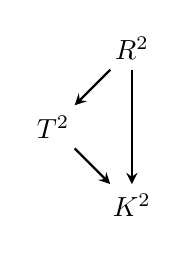
\begin{tikzpicture}[>=stealth, thick]

			% Nodes
			\node (X) at (0,2) {$\mathbb{R}^2$};
			\node (B) at (0,0) {$K^2$};
			\node (Bhat) at (-1,1) {$T^2$};

			% Arrows
			\draw[->] (X) -- (B);
			\draw[->] (X) -- (Bhat);
			\draw[->] (Bhat) -- (B);

		\end{tikzpicture}
	\end{center}
\end{frame}

\begin{frame}[c]{Nilpotent Holonomy}
	\begin{kulblock}{Corollary}
		Any integral affine structure on the 2-torus or the Klein bottle is complete.
	\end{kulblock}
\end{frame}

\begin{frame}[c]{Classification of Integral Affine Structures on $\mathbb{T}^2$ - $\pi_1(T^2) =  \mathbb{Z} \times \mathbb{Z}$}
	\begin{kulblock}{Theorem (K.N. Mishachev.3)}
		The possible generators for the affine holonomy group are
		\begin{enumerate}
			\item $(I, \begin{pmatrix}
					      a \\ c
				      \end{pmatrix})$ and $(I, \begin{pmatrix}
					      b \\ d
				      \end{pmatrix})$ with $\det(\begin{pmatrix}
					      a & b \\ c & d
				      \end{pmatrix}) \neq 0$ with $a,b,c,d \in \R$

			\item $(I, \begin{pmatrix}
					      a \\ 0
				      \end{pmatrix})$ and $(\begin{pmatrix}
					      1 & n \\ 0 & 1
				      \end{pmatrix}, \begin{pmatrix}
					      0 \\ b
				      \end{pmatrix})$ with $n \in \N$ and $a,b >0$
		\end{enumerate}
	\end{kulblock}
\end{frame}

\begin{frame}[c]
	Two integral affine structures of the first type are isomorphic if and only if
	\[
		X = G X' H
	\]
	where
	\[
		X = \begin{pmatrix} a & b \\ c & d \end{pmatrix},
		\qquad
		X' = \begin{pmatrix} a' & b' \\ c' & d' \end{pmatrix},
	\]
	and $G, H$ are some matrices from $\mathrm{GL}(2, \mathbb{Z})$.
\end{frame}

\begin{frame}[c]{Classification of Integral Affine Structures on $\mathbb{K}^2$ - $\pi_1(K^2) = \langle a,b \mid aba = b \rangle$}
	Let $A_1 = \begin{pmatrix}
			1 & n \\ 0 & 1
		\end{pmatrix}$, $A_2 = \begin{pmatrix}
			1 & n \\ 0 & 1
		\end{pmatrix}$ and $B_1 = \begin{pmatrix}
			1 & 0 \\ 0 & -1
		\end{pmatrix}$, $B_2 = \begin{pmatrix}
			0 & 1 \\ 1 & 0
		\end{pmatrix}$
	$B_3 = \begin{pmatrix}
			1 & 1 \\ 0 & -1
		\end{pmatrix}$
	\begin{kulblock}{Theorem (Daniele Sepe)}
		The possible generators for the affine holonomy group are
		\begin{enumerate}
			\item $(I, x\textbf{e}_2)$ and $(B_1, y\textbf{e}_1)$ with $x,y > 0$.
			\item $(A_1, x\textbf{e}_2)$ and $(B_1, y\textbf{e}_1 + x\textbf{e}_2)$ with $x,y > 0$.
			\item $(I, x(\textbf{e}_1 - \textbf{e}_2))$ and $(B_2, y\textbf{e}_2)$ with $x,y > 0$.
			\item $(A_2, x\textbf{e}_2)$ and $(B_3, y\textbf{e}_1 + \frac{n-1}{n}x\textbf{e}_2)$ with $2y \neq\frac{n-1}{n}x$ and $x>0$.
		\end{enumerate}
	\end{kulblock}
\end{frame}

\begin{frame}[c]{Lagrangian Fibrations}
	\begin{itemize}
		\item Whats next? - Lagrangian Fibrations over Compact Surfaces
	\end{itemize}
\end{frame}

